\chapter{Results and discussions}
\label{ch5:anchor:chapter}
\section{Introduction}
In this chapter, the results of the experimental tests conducted during this study are concisely presented and discussed. The variation and correlation observed are also presented. This chapter builds from the experimental method (Chapter \ref{ch4:anchor:chapter}).  Four tests were conducted as shown in the previous chapter, this was done to validate the objectives of the present study, which is to investigate the effect of mild steel, stainless steel, and \acrshort{hdpe} on \acrshort{afff} concentrate. 

To begin with, the \acrshort{ftir} results were analyzed to deduce the functional groups of the \acrshort{afff} concentrate. The \acrshort{tem} was used to determine the overall size and shape of the particles; the \acrshort{dls} was used to determine the particle size distribution; and lastly, the \acrshort{icp-aes} was used to identify the elemental composition within the \acrshort{afff} concentrate.

\section{AFFF concentrate infrared spectroscopy}
Figure \ref{ch5:figure:spectra} shows the \acrshort{ftir} spectra of the pure \acrshort{afff} concentrate compared to the \acrshort{afff} concentrate that has been exposed to the materials of interest. Their functionality in terms of stability, oxidation, and reactivity was revealed. Unsurprisingly, most of the chemical and functional groups appear within the group frequency of 4000–1500 cm$^{-1}$ wavenumber 4000-1500 cm$^{-1}$.

Referring to \ref{ch5:figure:spectra} (a), it can be observed that at the single bond region, broadband appears at 3355 cm$^{-1}$, which has been associated with a hydroxy group, the H-bonded OH stretch (\cite{krimm1986vibrational}). This functional group is responsible for enhancing the ability of the \acrshort{afff} concentrate surfactants to dissolve in water (\cite{coates1996interpretation}).  Medial alkyne C$\equiv$C stretch appears as a weak band at 2120 cm$^{-1}$; this is a vital distinguishing tool since very few organic compounds reveal an absorption in this region (\cite{bellamy1980infrared}). The medium band detected at 1637 cm$^{-1}$ can be assigned to alkenyl C=C stretch vibration. Interestingly, the fingerprint region also revealed quite a few functional groups. However, the methylene C-H bend and skeletal C-C vibrations can be disregarded since they appear in most organic compounds. Furthermore, the fluoro-compound C-F stretch at 1083 cm$^{-1}$ confirms the presence of fluorosurfactant in \acrshort{afff} concentrate. This C-F compound slightly shifted when the materials were immersed in \acrshort{afff} concentrate, with the largest shift observed when mild steel was immersed.

Referring to Figure \ref{ch5:figure:spectra} (b), which compares the \acrshort{ftir} spectra of pure \acrshort{afff} concentrate with \acrshort{afff} concentrate that has been exposed to materials of interest to deduce the significant shifts of functional groups in the single-bond region, a hydroxy group, H-bonded OH stretch, still appears in all the \acrshort{ftir} spectra. However, there is a strange absorption peak of aldehyde C-C stretching that appears in \acrshort{afff} concentrate after \acrshort{hdpe} and stainless steel were immersed at bands 2710 and 2697 cm$^{-1}$, respectively (\cite{lin1991handbook}). This may indicate an interaction between the \acrshort{afff} concentrate and these two materials. Moreover, there is a significant shift that can be observed in the triple bond region at bands 2056 and 2060 cm$^{-1}$ for exposed \acrshort{hdpe} and stainless steel \acrshort{afff} concentrate, respectively. Consequently, this shift confirms the presence of isothiocyanate N=C=S stretching, which is a very unusual functional group, especially in organic compounds

It can be clearly observed that there are minor shifts in the functional groups. However, these minor shifts can be subsequently used to predict the reaction of the materials with the \acrshort{afff} concentrate in the long term. This is a very useful prediction technique since, in the present study, these materials were immersed in \acrshort{afff} concentrate for only five months. Furthermore, the major reaction in the real world could take years. Figure \ref{ch5:figure:materials} (a-c) in Section \ref{ch5:anchor:section:spectroscopy} compares the \acrshort{ftir} spectra of the pure mild steel, stainless steel, and \acrshort{hdpe} to others that have been immersed in \acrshort{afff} concentrate. This was done to further examine and validate the functional group shifts on the exposed materials of interest.

\begin{figure}[H]
\centering

\begin{subfigure}{.45\textwidth}
    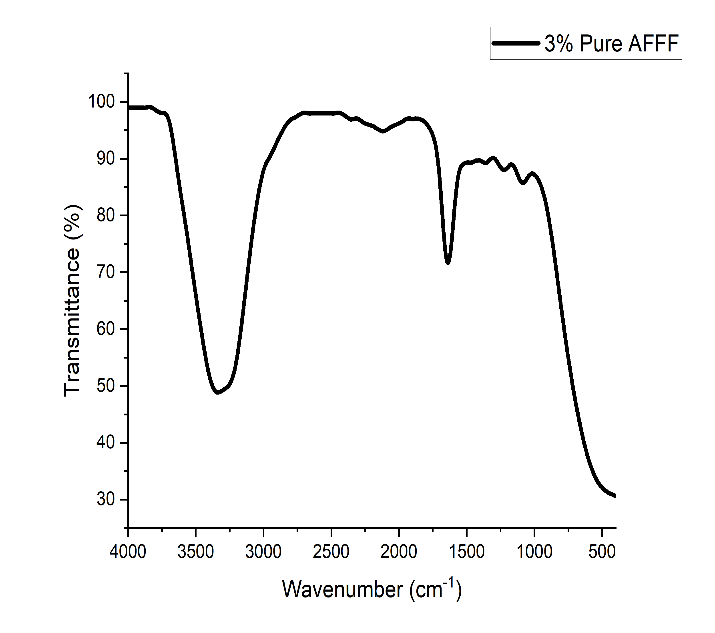
\includegraphics[width=\textwidth]{ftir_spectra.png}
    \caption{}
    \label{ch5:figure:spectra:a}
\end{subfigure}
\begin{subfigure}{.45\textwidth}
    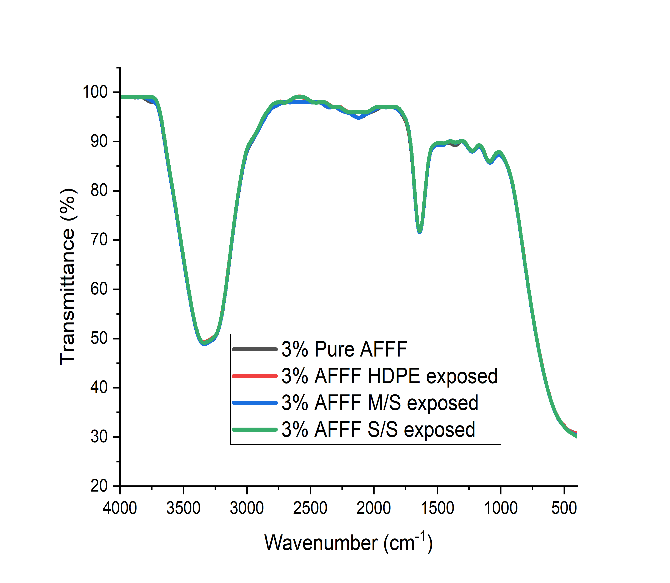
\includegraphics[width=\textwidth]{comparison.png}
    \caption{}
    \label{ch5:figure:spectra:b}
\end{subfigure}

\caption{Comparisons Pure AFFF spectra (a) with the other materials after they were immersed (b).}
\label{ch5:figure:spectra}
\end{figure}

\section{Infrared spectroscopy of HDPE, Mild steel, and Stainless steel}  
\label{ch5:anchor:section:spectroscopy}

The \acrshort{ftir} spectra of the materials of interest were conducted to substantiate the minor shifts of the functional group on the exposed \acrshort{afff} concentrate. Figure \ref{ch5:figure:materials} (a-c) shows the \acrshort{ftir} spectra of the materials of interest. The reactivity of \acrshort{afff} concentrate with the materials was of particular interest. It can be observed from Figure \ref{ch5:figure:materials} (a-c) that there are significant shifts in functional groups. In Figure \ref{ch5:figure:materials} (a), the O-H stretching, which can be observed at 3583 cm$^{-1}$ in pure \acrshort{hdpe}, shifted to a wavenumber of 3817 cm$^{-1}$ when the materials were immersed in \acrshort{afff} concentrate (\cite{mudunkotuwa2014atr}). In pure \acrshort{hdpe}, a strong amine N-H stretching at 3358 cm$^{-1}$ can be seen, which shifts to a broad band at 3406 cm$^{-1}$ in immersed concentrate (\cite{mohamed2017fourier}).

\begin{figure}[H]
\centering

\begin{subfigure}{.45\textwidth}
    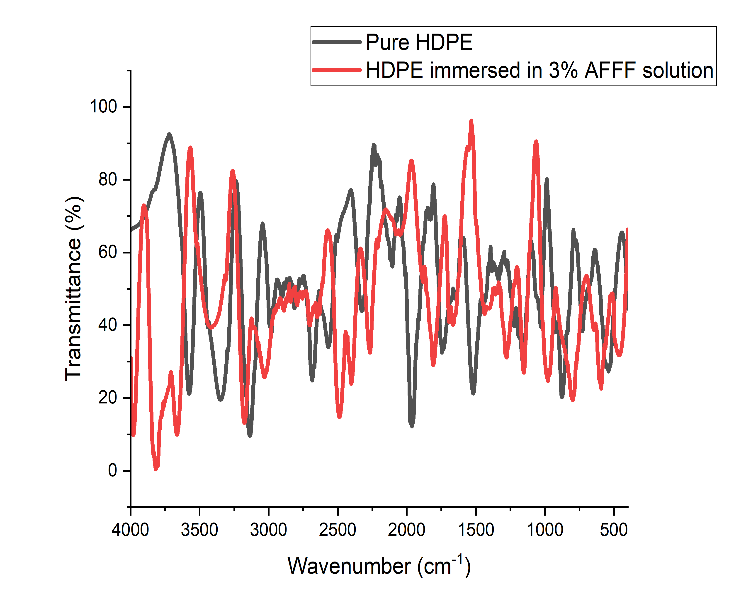
\includegraphics[height=6cm, width=\textwidth]{pure_hdpe_ftir_spectra.png}
    \caption{}
\end{subfigure}
\begin{subfigure}{.45\textwidth}
    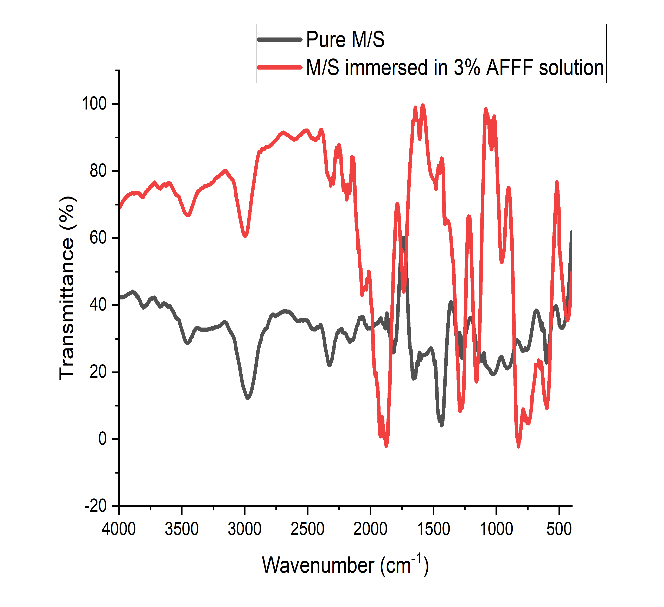
\includegraphics[height=6cm, width=\textwidth]{pure_ms_ftir_spetra.png}
    \caption{}
\end{subfigure}
\begin{subfigure}{.45\textwidth}
    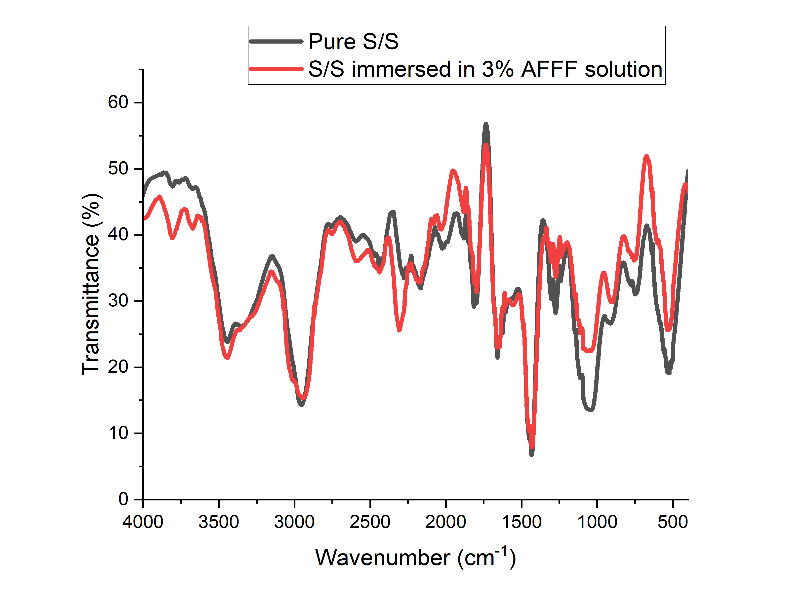
\includegraphics[width=\textwidth]{pure_ss_ftir_spectra.png}
    \caption{}
\end{subfigure}

\caption{FTIR spectra, comparing various materials.}
\label{ch5:figure:materials}
\end{figure}

\section{Transmission electron microscopy (TEM)}
The JEOL JEM-1010 \acrshort{tem} used for the present study is equipped with highly integrated technology. The 40 kV to 100 kV operating voltage range is suitable for applications in material science. Because of its low operating voltage and unique objective pole piece design, the JEM-1010 is a \acrshort{tem} with outstanding contrast (\cite{klein2011transmission}). Additionally, it has a 2K x 2K AMT CCD camera for taking digital images. Using high resolution (HR) and electron diffraction imaging, the \acrshort{tem} was able to provide overall particle shape, a large variety of particles, and a visual overall of the particle shape of the \acrshort{afff} concentrate samples. 

The \acrshort{tem} images of pure \acrshort{afff} concentrate are shown in Figure \ref{ch5:figure:pure_afff_images}. These are utilized as a benchmark and compared to the immersed concentrate to observe any critical particle changes. All the samples depict the HR and electron diffraction images in various parts. This was done to understand the overall particle shape of the concentrate before making any conclusions.

\begin{figure}[H]
\centering
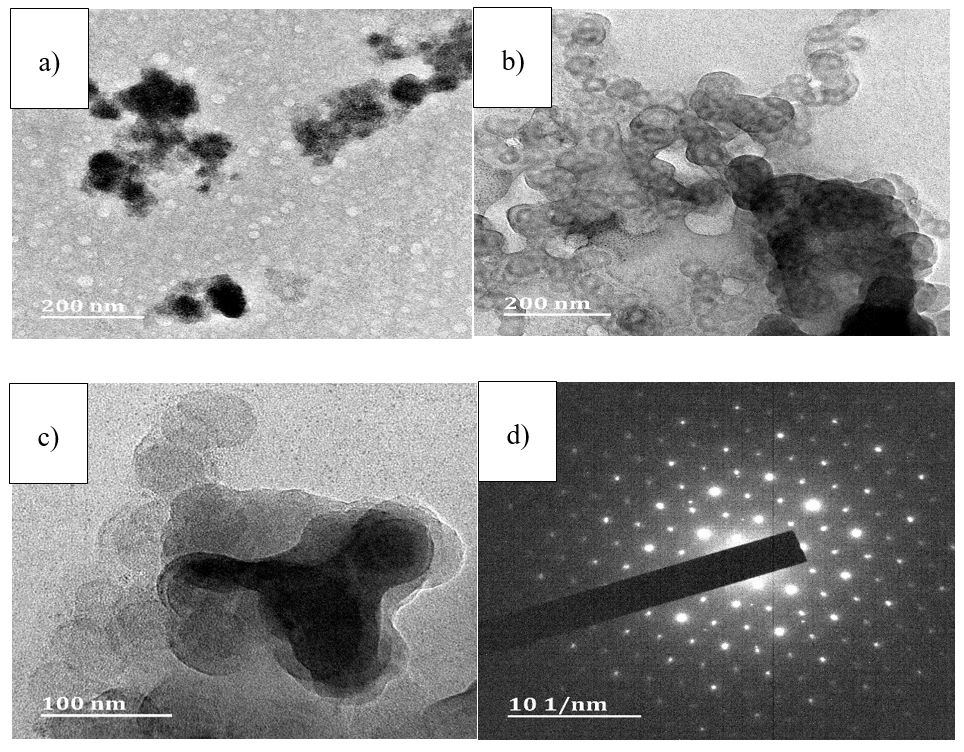
\includegraphics[width=.88\textwidth]{new_fig_4.jpg}

\caption{HR (a-c) and electron diffraction images (d) of pure AFFF concentrate.}
\label{ch5:figure:pure_afff_images}
\end{figure}

It can be observed from Figure \ref{ch5:figure:pure_afff_images} (d) that the electron diffraction image of pure \acrshort{afff} concentrate provides numerous spots that are aligned in a particular direction. This is a demonstration that the concentrate in a pure state has a single crystalline structure. This shows that the concentrate has uniform properties and is more stable in its pure form (\cite{bandyopadhyay2019fabrication}). Moreover, Figure \ref{ch5:figure:pure_afff_images} (a-c) reveals that the particles of pure \acrshort{afff} concentrate are scattered along the concentrate. This might be caused by the collision of two or more repelling particles within the concentrate (\cite{pyrz2008particle}). Figures \ref{ch5:figure:mild_steel_images} - \ref{ch5:figure:hdpe_images} depict the HR and electron diffraction images when various materials were immersed in \acrshort{afff} concentrate. 
  
\begin{figure}[H]
\centering

\includegraphics[width=.9\textwidth]{electron_diffraction_images_of_pure_AFFF_concentrate_4-8.png}

\caption{HR (a-c) and electron diffraction images (d) of AFFF concentrate immersed in mild steel.}
\label{ch5:figure:mild_steel_images}
\end{figure}

\begin{figure}[H]
\centering

\includegraphics[width=.9\textwidth]{electron_diffraction_images_of_pure_AFFF_concentrate_8-12.png}

\caption{HR (a-c) and electron diffraction images (d) of AFFF concentrate immersed in stainless steel.}
\label{ch5:figure:stainless_steel_images}
\end{figure}

\begin{figure}[H]
\centering

\includegraphics[width=.9\textwidth]{electron_diffraction_images_of_pure_AFFF_concentrate_12-16.png}

\caption{HR (a-c) and electron diffraction images (d) of AFFF concentrate immersed in HDPE.}
\label{ch5:figure:hdpe_images}
\end{figure}

The overall crystal structure and the difference in particle shape for the three samples compared to a pure \acrshort{afff} sample were studied. Although the present \acrshort{tem} analyses are not able to provide the precise particle sizes of the samples, they nonetheless provide a significant overall change in the crystal structure. Figure \ref{ch5:figure:pure_afff_images} revealed that in a pure state, \acrshort{afff} concentrate posses revealed that in a pure state, \acrshort{afff} concentrate possesses a single crystalline structure. However, when studying Figures \ref{ch5:figure:mild_steel_images} - \ref{ch5:figure:hdpe_images}, it is observed that the exposed \acrshort{afff} concentrate has critically changed to a polycrystalline structure. When closely inspecting the electron diffraction images of these samples, this is seen in Figures \ref{ch5:figure:mild_steel_images} - \ref{ch5:figure:hdpe_images} (d). The concentrated circular rounds imply that all these materials are polycrystalline. This is confirmed by the morphology (particles, grains, and crystallites), as several grains are observed in Figures \ref{ch5:figure:mild_steel_images} - \ref{ch5:figure:hdpe_images}. These grains are separated by grain boundaries and have random crystallographic orientations. It can be further observed that Figure \ref{ch5:figure:mild_steel_images} has more grains compared to Figures \ref{ch5:figure:stainless_steel_images} and \ref{ch5:figure:hdpe_images}. Consequently, this implies that most of the crystal structural changes occurred when mild steel was immersed in \acrshort{afff} concentrate.

When comparing the differences topographically (structure and shape), it can be observed in Figure \ref{ch5:figure:pure_afff_images} that the particles for pure \acrshort{afff} concentrate are scattered and distributed along the concentrate. However, when closely observing Figures \ref{ch5:figure:mild_steel_images} - \ref{ch5:figure:hdpe_images}, it can be seen that the particles for these samples are concentrated in one area, especially in Figure \ref{ch5:figure:mild_steel_images}. As a result, this demonstrates that when the materials of interest were immersed in \acrshort{afff} concentrate, there was a structural and shape particle change. The alteration in crystal structure and particle shape in \acrshort{afff} concentrate complements the shifts in functional groups obtained using \acrshort{ftir}. \cite{an2018effect} experimentally investigated the effect of the particle shape on the viscosity of the liquid. Their results indicated that the spherical particles have a lower viscosity, and any other particle shape will result in a higher viscosity. In addition, a change in any additives in \acrshort{afff} concentrate will affect the foam drainage time. It should be noted that the causes of these alterations are not known as of yet. However, conclusive results and interpretations are detailed in Sections \ref{ch5:anchor:section:dls} and \ref{ch5:anchor:section:analysis} using the \acrshort{dls} and elementary analysis to validate the vital information provided by \acrshort{ftir} and \acrshort{tem}.

\section{Dynamic light scattering (DLS)}
\label{ch5:anchor:section:dls}
In this section, an in-depth understanding of the cause of crystal structure and particle shape changes within the \acrshort{afff} concentrate and the impact these changes possess on the performance parameters are discussed. This is achieved by evaluating the particle size and particle size distribution of \acrshort{afff} concentrate by measuring the hydrodynamic diameter (Z-average) of any present particles in units of nanometers (nm) using a \acrshort{dls} technique. \acrshort{dls} is a noninvasive technique that depends on the particles moving randomly as a result of collisions with the solvent molecules (Brownian motion). As a result, only particles suspended in a liquid may be categorized (\cite{machhi2021effect}). The determination of particle size and size distribution is essential because these characteristics have a large effect on the properties of the \acrshort{afff} concentrate, including its mechanical stability, foaming ability, and a viscosity (\cite{de2017detection}).

\subsection{Particle size analysis}
\label{ch5:anchor:section:size_analysis}

Figure \ref{ch5:figure:samples} depicts the four samples used during the \acrshort{dls} analysis, where 1, 2, and 3 are \acrshort{afff} concentrates when mild steel, stainless steel, and \acrshort{hdpe}, respectively, have been immersed. Sample 4 is a pure \acrshort{afff} concentrate for benchmark purposes. Table \ref{ch5:table:sizes} shows the summary of the results for average particle sizes for the four samples in nm.
  
\begin{figure}[H]
    \centering
    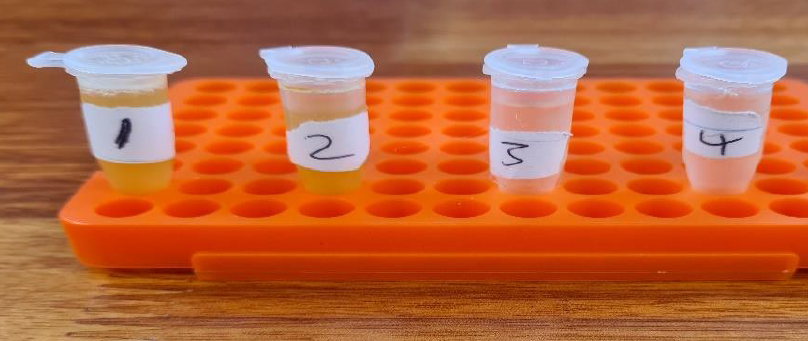
\includegraphics[width=.7\textwidth]{samples_used_during_the_dls_analysis.png}
    \caption{Samples used during the DLS analysis.}
    \label{ch5:figure:samples}
\end{figure}

\begin{table}[H]
\renewcommand{\arraystretch}{2}

\caption{Summary of average particle sizes.}

\begin{tabularx}{\textwidth}{ XX }
\hline
\textbf{SAMPLE ID} & \textbf{Z-AVERAGE (D)} \\
\hline
\textbf{1} & 660.7 nm \\
\textbf{2} & 4.892 nm \\
\textbf{3} & 4.036 nm \\
\textbf{4} & 3.586 nm \\
\hline
\end{tabularx}

\label{ch5:table:sizes}
\end{table}

It can be observed from Table \ref{ch5:table:sizes} that there have been changes in particle diameter. The pure \acrshort{afff} concentrate has an average particle size of 3.586 nm, which is a very small particle size. However, when comparing this to samples 2 and 3, it can be observed that there is a slight difference or change. To be precise, the change in Z-average is around 1.306 nm at most. At this point, it is not known if these changes are slight enough to not affect the properties of \acrshort{afff} concentrate. Sample 1, in Table \ref{ch5:table:sizes}, shows a major change in particle size. Sample 1 has an average particle size of 660.7 nm, which is way above the other three samples by about 655.808 nm at most. This difference is extremely surprising and has some implications. \cite{koca2018effect} studied the effect of particle size on the properties of nanofluids. They discovered that larger particles have a slower diffusion speed than smaller ones. In a fluid, a particle's translational diffusion coefficient and hydrodynamic diameter are related by the Stokes-Einstein equation (\cite{an2018effect}), as demonstrated by Equation (\ref{ch5:equation:stokes_einstein}).

It can be observed from Table \ref{ch5:table:sizes} that there have been changes in particle size diameter. The pure \acrshort{afff} concentrate has an average particle size of 3.586 nm, which is a very small particle size. However, when comparing this to sample 2 and 3 it can be observed that there is a slight difference or change. To be precise, the change in Z-average is around 1.306 nm at most. At this point, it is not known if these changes are slight in such a way that they do not have any effect on the properties of \acrshort{afff} concentrate. Sample 1, in Table \ref{ch5:table:sizes} shows a major change in particle size. Samples 1 has an average particle size of 660.7 nm, which is way above the other three samples by about 655.808 nm at most. This difference is extremely surprising and obviously has some implications. As a matter of fact, larger particles have a gradual diffusion speed than smaller particles. In a fluid, a particle's translational diffusion coefficient and hydrodynamic diameter are related by the Stokes-Einstein equation (\cite{lin1991handbook}), as demonstrated by equation (\ref{ch5:equation:stokes_einstein}).

\begin{equation}
    D_T=\frac{K_bT}{b\pi \eta R_h}
    \label{ch5:equation:stokes_einstein}
\end{equation}

\begin{doublespace}
Where, \\
$D_T\ is\ the\ transitional\ diffusion\ coefficient\ in\ \nicefrac{m^2}{s}$ \\
$R_H\ is\ the\ hydrodynamic\ radius\ in\ m$ \\
$K_b\ is\ the\ Boltzmann\ constant\ in\ \nicefrac{J}{K}$ \\
$T\ is\ the\ Temperature\ in\ K$ \\
$\eta\ is\ the\ viscosity\ of\ the\ medium\ in\ \nicefrac{Ns}{m^2}$ \\
$b\ is\ the\ constant\ that\ depends\ on\ the\ size\ of\ the\ diffusing\ molecules$ \\
\end{doublespace}

As a matter of fact, for \acrshort{afff} stability, rapid diffusion of fluorosurfactant molecules is required. It can be observed from Equation (\ref{ch5:equation:stokes_einstein}) that the rate of diffusion is inversely proportional to the particle size. However, it also depends on the surface area and temperature. For the present study, all the samples were exposed to the same temperature (atmospheric) for an equitable comparison. This is a demonstration that once \acrshort{afff} concentrate has been in contact with mild steel, it decreases its diffusion rate rapidly and thus decreases the foaming stability of \acrshort{afff}.  On the other hand, the Z-average (particle size diameter) results demonstrate that when stainless steel and \acrshort{hdpe} have been immersed in \acrshort{afff} concentrate, there are slight differences in particle diameter when compared to pure \acrshort{afff} concentrate. When visually observing the numbers, the difference looks slight. On the contrary, the percentage increase calculations demonstrate a relatively large difference. The fundamental equation is given as:

\begin{doublespace}
\begin{eqnarray}
    \label{ch5:equation:stainless_steel}
    \%Increase &=& \frac{D_s - D_O}{3.586} \times 100 \\ 
    \nonumber &=& \frac{4.892 - 3.586}{3.586}\times 100 \\
    \nonumber &=& 36.419\%
\end{eqnarray}
\end{doublespace}

It is possible to calculate the percentage increase in particle size for the \acrshort{afff} concentrate when stainless steel was immersed.

\begin{doublespace}
Where, \\
$D_s\ is\ the\ particle\ size\ diameter\ of\ sample\ 2\ in\ nm$ \\
$D_O\ is\ the\ particle\ size\ diameter\ of\ sample\ 4\ in\ nm$ \\
\end{doublespace}

The same formula employed in Equation (\ref{ch5:equation:stainless_steel}) can be used to calculate the percentage increase in particle diameter for the \acrshort{afff} concentration when \acrshort{hdpe} was immersed. 

\begin{doublespace}
\begin{eqnarray}
    \label{ch5:equation:hdpe}
    \%Increase &=& \frac{D_s - D_O}{D_O} \times 100 \\ 
    \nonumber &=& \frac{4.036 - 3.586}{3.586}\times 100 \\
    \nonumber &=& 12.549\% 
\end{eqnarray}
\end{doublespace}
 
\begin{doublespace}
Where, \\
$D_s\ is\ the\ particle\ size\ diameter\ of\ sample\ 2\ in\ nm$ \\
$D_O\ is\ the\ particle\ size\ diameter\ of\ sample\ 4\ in\ nm$ \\
\end{doublespace}

It can be seen from Equation (\ref{ch5:equation:stainless_steel}) that the particle size percentage change is 36.419\% when stainless steel is immersed in \acrshort{afff} concentrate. This can be regarded as a huge increase since there is more than a quarter (1/4) difference between the two particles. When analyzing Equation (\ref{ch5:equation:hdpe}), it can be observed that when \acrshort{hdpe} was immersed in AFF concentrate, the particle size had an average change of 12.549 nm. This is a much smaller percentage compared to 36.419 nm, with a difference of 23.87 nm. However, it cannot be guaranteed that it does not affect the foaming ability of \acrshort{afff} concentrate. At this moment, there are still doubts regarding the effects of these materials on \acrshort{afff} concentrate. However, the analysis of the particle size distribution (PSD) and element composition will be conducted in Sections \ref{ch5:anchor:section:psd} and \ref{ch5:anchor:section:analysis}, respectively, for further validation.

\subsection{Particle size distribution (PSD) analysis}
\label{ch5:anchor:section:psd}
\acrshort{dls} is a widely accepted method to evaluate the hydrodynamic size of concentrate particles. The \acrshort{dls} particle size results can be represented using volume, number, and intensity. However, as stated in the international standard (\acrshort{iso} 22412:2017), intensity-based results are the most reliable parameters provided by \acrshort{dls} to describe particle size and particle size distribution (PSD) (\cite{ramirez2021characterization}). As a consequence, the intensity-based results were opted for in the present research work to analyze the PSD of pure \acrshort{afff} concentrate and \acrshort{afff} concentrate after the three materials were immersed. A comparison in size distribution is then made to understand the influence of each material on the properties of \acrshort{afff} concentrate. PSD is essential for understanding the chemical and physical properties of a sample. The particles within the \acrshort{afff} concentrate have similar sizes and are relatively uniform. The PSD curve of the pure \acrshort{afff} concentrate plotted by intensity is shown in Figure \ref{ch5:figure:pure_afff}. This PSD curve is used to compare the alteration in PSD of \acrshort{afff} concentrate when various materials were immersed.

\begin{figure}[H]
    \centering
    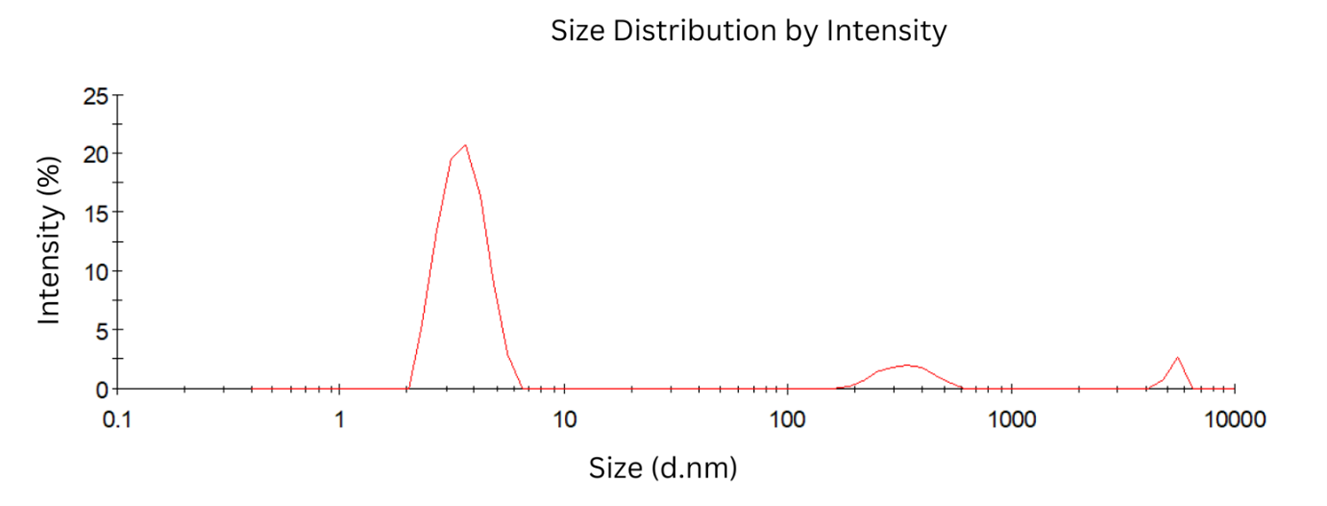
\includegraphics[width=\textwidth]{particle_size_distribution_of_pure_afff_solution.png}
    \caption{Particle size distribution of pure AFFF concentrate.}
    \label{ch5:figure:pure_afff}
\end{figure}

It can be observed from Figure \ref{ch5:figure:pure_afff} that the particle size distribution curve shows that the peaks are divided into three intensities. As expected, the major peak is at a particle size of 3.586 nm, as previously shown in Table \ref{ch5:table:sizes}, and the second and third peaks can be estimated at 350 and 5500 nm, respectively. \cite{de2017detection} studied the particle size distribution of aqueous concentrate. They demonstrated that the aqueous concentrate with a narrow PSD was able to disperse easily. Similarly, it can be seen from Figure \ref{ch5:figure:pure_afff} that the first peak is very narrow. As expected, this is evidence that in a pure state, \acrshort{afff} concentrate can disperse or spread rapidly over a large surface area.

\begin{figure}[H]
    \centering
    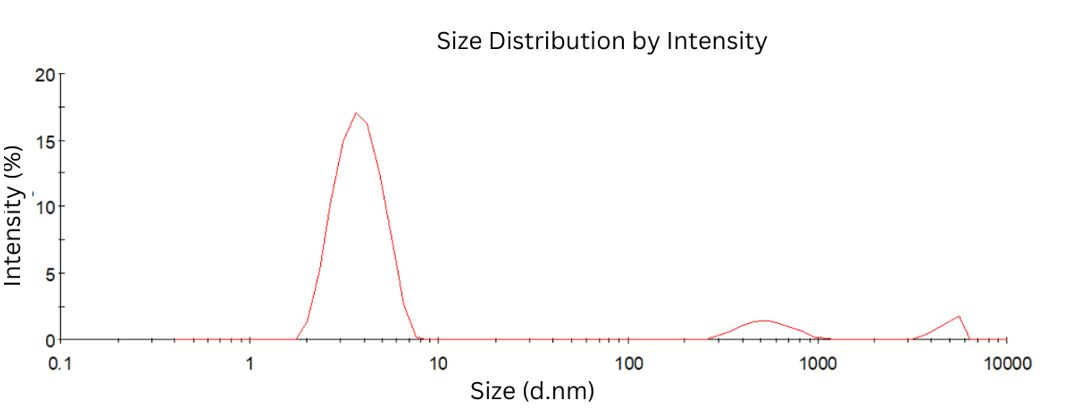
\includegraphics[width=.95\textwidth]{graph_5_9.jpg}
    \caption{Particle size distribution of AFFF concentrate when stainless steel was immersed.}
    \label{ch5:figure:stainless_steel}
\end{figure}

Referring to Figure \ref{ch5:figure:stainless_steel}, it is observed that the \acrshort{afff} concentrate possesses three peaks. This is precisely the same observation as in Figure \ref{ch5:figure:pure_afff}. Unsurprisingly, the main peak can be attributed to a particle size of 4.892 nm. Moreover, it can be seen from Figure \ref{ch5:figure:stainless_steel} that the main peak has a narrow PSD. However, when closely observed, it is slightly wider compared to Figure \ref{ch5:figure:pure_afff}. This demonstrates that stainless steel did not cause any critical alteration of PSD within the AFF concentrate, as it is still able to disperse easily. This is a validation that stainless steel does not influence the spreading ability of \acrshort{afff}. This further concludes that the minor particle size alteration discussed in Section \ref{ch5:anchor:section:size_analysis} and Equation (\ref{ch5:equation:stainless_steel}) does not have a significant impact on the diffusion rate of fluorosurfactant molecules.   
  
\begin{figure}[H]
    \centering
    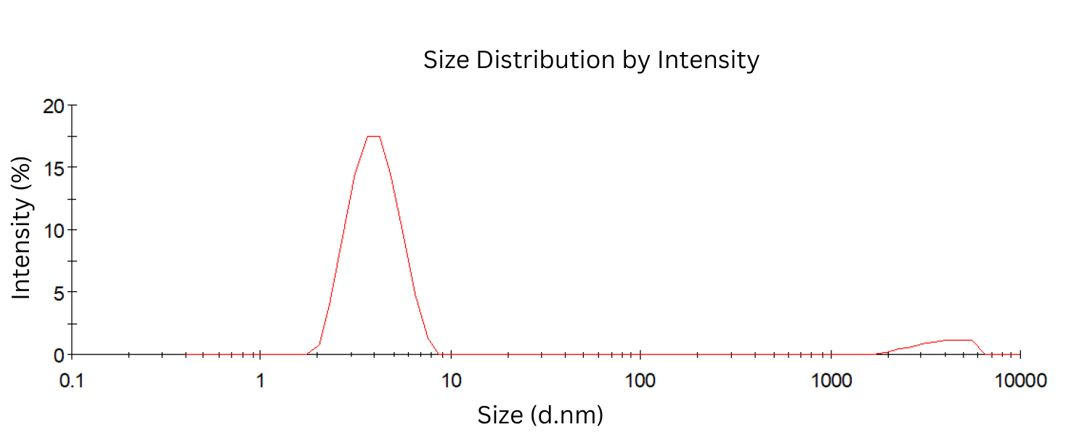
\includegraphics[width=.95\textwidth]{graph_5_10.jpg}
    \caption{Particle size distribution of AFFF concentrate when HDPE was immersed.}
    \label{ch5:figure:hdpe}
\end{figure}

It can be observed from Figure \ref{ch5:figure:hdpe} that the PSD curve consists of peaks that are divided into two intensities. This is in contrast to Figures \ref{ch5:figure:pure_afff} and \ref{ch5:figure:stainless_steel}, where the peaks were divided into three intensities. The major peak can be associated with a particle size of 4.036 nm, whereas the other peak can be estimated at 5000 nm. When observing the broadness of the major peak, it can be noticed that it is wider than the peak in Figure \ref{ch5:figure:pure_afff} and almost the same size as Figure \ref{ch5:figure:stainless_steel}. This, however, can be considered a narrow peak. Moreover, this provides sufficient evidence that \acrshort{hdpe} does not alter the PSD within the pure \acrshort{afff} concentrate, which suggests that the dispersion rate is not affected. This further concludes that the minor particle size alteration discussed in Section \ref{ch5:anchor:section:analysis} and Equation (\ref{ch5:equation:hdpe}) does not have a significant impact on the diffusion rate of fluorosurfactant molecules.  
  
\begin{figure}[H]
    \centering
    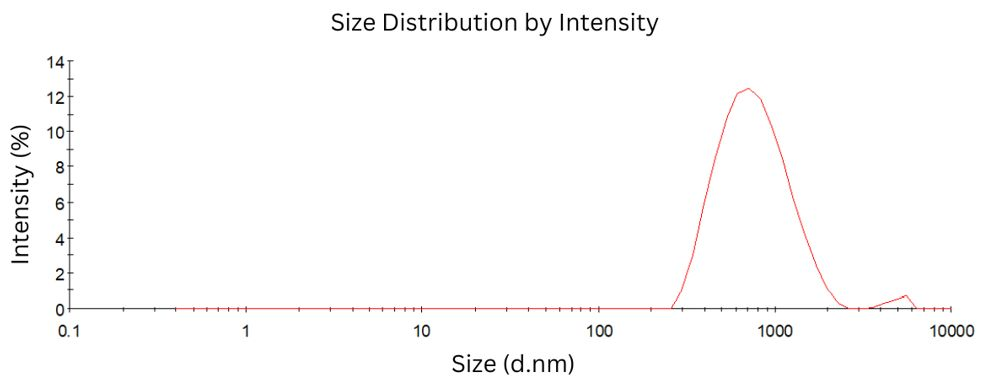
\includegraphics[width=.95\textwidth]{graph_5_11.jpg}
    \caption{Particle size distribution of AFFF concentrate when mild steel was immersed.}
    \label{ch5:figure:mild_steel}
\end{figure}

Surprisingly, Figure \ref{ch5:figure:mild_steel} depicts a distinct PSD compared to Figures \ref{ch5:figure:pure_afff}-\ref{ch5:figure:hdpe}. It can be observed that Figure \ref{ch5:figure:mild_steel} reveals peaks that are divided into two intensities. These peaks can be associated with particle sizes of 660.7 nm, whereas the other peak can be estimated at 5500 nm. Due to the large difference in sizes between these two peaks, they can be generally regarded as major and minor peaks, respectively. It is interesting to note that Figure \ref{ch5:figure:mild_steel} possesses a wide major peak compared to all previous peaks illustrated in Figures \ref{ch5:figure:pure_afff}-\ref{ch5:figure:hdpe}. This is an indication that there has been a sensitive reaction between mild steel and \acrshort{afff} concentrate. Moreover, this demonstrates that the spreading ability of the concentrate has been reduced. This could be caused by several parameters, such as an increase in viscosity that causes the concentrate to be slightly thicker. However, it is well known that viscosity is largely dependent on the shape of the particles, where any deviation from the spherical shape of the particle increases viscosity (\cite{karau1997influence}). Nevertheless, it is noticed in Figure \ref{ch5:figure:mild_steel} that the alteration in PSD can have a slight impact on the spreading capability of the aqueous concentrate. 

\section{Wet chemical analysis}
\label{ch5:anchor:section:analysis}
As aforementioned, the \acrshort{icp-aes} was used to identify both the amounts and major concentrations of elements within the exposed \acrshort{afff} concentrate and benchmark these with the standard quantities and qualities. The alterations in elements or composition can immensely affect the properties, hence the performance of \acrshort{afff} during firefighting circumstances. The concrete results are provided in this section, and conclusive information is drawn regarding the severity of mild steel, stainless steel, and \acrshort{hdpe} on the performance parameters of \acrshort{afff}. In addition, the elementary results are more reliable as they provide the precise elements that are present within the \acrshort{afff} concentrate before and after the materials were immersed. Thus, they validate the previous results of the analyses conducted using \acrshort{ftir}, \acrshort{tem}, and \acrshort{dls}.

\subsection{Elemental componsition analysis}
For the present research, the elements were analyzed based on the importance of the role they possess within the \acrshort{afff} concentrate. To begin with, \acrshort{afff} is water-based and commonly contains a hydrocarbon-based surfactant such as sodium alkyl sulfate. They discovered that the presence of sodium and sulphur within these fluids is responsible for the stable foam formation. \cite{yu2020formation} studied the formation of stable aqueous foams. They experimentally demonstrated that the presence of sodium and sulphur within the aqueous solution is responsible for the stable foam formation. As a matter of fact, for stable foam formation, there must be less surface tension in the water. This is mostly accomplished by increasing the sodium alkyl sulfate concentration. As a consequence, sodium and sulphur were the primary elements of interest. Other elements were also analyzed at a later stage, and their impacts on the performance parameter of \acrshort{afff} were concisely discussed. Table \ref{ch5:table:chemical_elements_1} depicts the elemental composition results of the pure \acrshort{afff} concentrate and the other when mild steel, stainless steel, and \acrshort{hdpe} were immersed. The entire elemental composition results are depicted in Figures \ref{appendix:samples_1-3} and \ref{appendix:sample4} in the appendices for validation purposes.

\newcolumntype{Y}{>{\centering\arraybackslash}X}

\begin{table}[H]
\renewcommand{\arraystretch}{2}
\caption{Chemical elements of AFFF concentrate.}

\begin{tabularx}{\textwidth}{*{6}{Y}}
\hline
Element & Chemical symbol & \multicolumn{4}{c}{Composition in PPM} \\
& & \multicolumn{4}{c}{Sample ID:} \\
\hline
& & 1 & 2 & 3 & 4 \\
Sodium & Na & 2302 & 2332 & 2349 & 2354 \\
Sulphur & S & 92 & 89 & 94.2 & 94.7 \\
\hline
\end{tabularx}

\label{ch5:table:chemical_elements_1}
\end{table}

Referring to Table \ref{ch5:table:chemical_elements_1}, samples 1-3 are the \acrshort{afff} concentrate after mild steel, stainless steel, and \acrshort{hdpe} were immersed, respectively, with sample 4 being the pure \acrshort{afff} concentrate. From Table 4, it can be observed that in a pure state, \acrshort{afff} concentrate has 2354 and 94.7 parts per million (ppm) of sodium and sulphur, respectively. When observing closely, it is seen that the sodium in pure \acrshort{afff} concentrate (sample 4) decreases gradually. To be precise, the sodium is reduced by 5, 22, and 52 ppm, respectively, from the pure \acrshort{afff} concentrate. This indicates that the sodium composition of the \acrshort{afff} concentrate is reduced when it is exposed to the materials of interest. Moreover, it can be observed that the amount of reduction in sodium is diverse in all samples. This further demonstrates that the severity of the effects caused by the materials on the foam’s stability varies greatly.

Similar occurrences can be observed with sulphur. Referring to Table \ref{ch5:table:chemical_elements_1}, it is observed that the elemental composition of sulphur in pure \acrshort{afff} decreases when it reacts with various materials. Consequently, it is evident that the reaction of the three materials with the \acrshort{afff} concentrate reduces the surfactants (sodium alkyl sulfate). This increases the surface tension of the water within the concentrate, reducing the stability of the foam. Moreover, it can be seen that the sodium alkyl sulphate was immensely reduced when the \acrshort{afff} concentrate was in contact with mild steel (Sample 1). These findings correlate with \acrshort{ftir} analyses, which confirmed the presence of isothiocyanate N=C=S stretching on the triple bond region at bands 2056 and 2060 cm$^{-1}$. This functional group confirmed the presence of sulphur in the \acrshort{afff} concentrate when \acrshort{hdpe} and stainless steel were immersed, but sulfur did not appear in the \acrshort{afff} concentrate when mild steel was immersed.

In addition, the elementary findings further correlate with the gradual diffusion rate of surfactants due to large particles discussed in \ref{ch5:anchor:section:size_analysis}. These findings are evidence that stainless steel and \acrshort{hdpe} have a minimal effect on the foam ability and foam stability of \acrshort{afff}. They further demonstrate that mild steel has a severe impact on the two performance parameters of \acrshort{afff} due to the chemical elements’ reactions with surfactants. However, further studies should be conducted to determine the precise causes of the negative effects of these materials, as this research is limited to the impacts or effects of the materials in \acrshort{afff} concentrate. In this way, it will be uncomplicated to optimize these materials in such a way that they are compatible with the \acrshort{afff} concentrate.

The \acrshort{icp-aes} used for the present research was not able to detect organic compounds. However, the functional groups revealed by \acrshort{ftir} spectra were sufficient to provide the key variations of the elements within the \acrshort{afff} concentrate. The shifting of the C-F stretch observed in Table \ref{ch5:table:chemical_elements_1} confirmed that the materials of interest also affect the fluorine content that is present within the PFAS in \acrshort{afff} concentrate. This alteration of fluorine is a huge setback for the performance parameters of \acrshort{afff}. PFAS are responsible for forming an aqueous film on fire fuels, which effectively suffocates them by creating a barrier to any oxygen and cooling them to prevent hot fuels from reigniting (\cite{hinnant2020characterizing}). Consequently, the alteration of fluorine within the \acrshort{afff} concentrate greatly reduces the blanketing capabilities during firefighting. It is well known that PFAS are harmful to the environment and humans (carcinogenic). However, the \acrshort{afff} is primarily chosen for its effective extinguishing capabilities due to PFAS. This implies that any alteration of fluorine within the \acrshort{afff} concentrate yields unfavourable outcomes. Other vital elements that influence the performance of \acrshort{afff} are listed in Table \ref{ch5:table:chemical_elements_2} and concisely discussed.

\begin{table}[H]
\renewcommand{\arraystretch}{2}
\caption{Chemical elements of AFFF concentrate}

\begin{tabularx}{\textwidth}{*{6}{Y}}
\hline
Element & Chemical symbol & \multicolumn{4}{c}{Composition in PPM} \\
& & \multicolumn{4}{c}{Sample ID:} \\
\hline
& & 1 & 2 & 3 & 4 \\
Aluminium & Al & 0.9 & 0.2 & 0.5 & 1.1 \\
Calcium & Ca & 46 & 07 & 10 & 6.9 \\
Iron & Fe & 132 & 58 & 3.7 & 2.5 \\
Potassium & K & 04 & 03 & 2.8 & 2.4 \\
Magnesium & Mg & 27 & 03 & 2.4 & 2.3 \\
Silicon & Si & 07 & 07 & 11 & 10.6 \\
\hline
\end{tabularx}

\label{ch5:table:chemical_elements_2}
\end{table}

Referring to Table \ref{ch5:table:chemical_elements_2}, it is noticed that the iron content observed in pure \acrshort{afff} concentrate increased when various materials were immersed. Initially, the iron concentration was 2.5 ppm; it then increased to 3.7, 58, and 132 ppm when \acrshort{hdpe}, stainless steel, and mild steel were immersed, respectively. In general, the increase in the iron element predominantly implies the degradation or wearing of the material (\cite{mcarthur2004engineering}). Consequently, this demonstrates that mild steel degrades immensely when in contact with the \acrshort{afff} concentrate, as the iron element increases by 129.5 ppm. This is evidence that there is a severe reaction between \acrshort{afff} concentrate and mild steel. The obvious reason for this could be the initiation of corrosion in mild steel when it was first exposed to environmental conditions before immersion in \acrshort{afff} concentrate. On the other hand, \acrshort{hdpe} and stainless steel underwent a similar process, with severity being a major difference. The iron element increased by 1.2 and 55.5 ppm when \acrshort{hdpe} and stainless steel reacted with \acrshort{afff} concentrate, respectively.

The other elements, such as calcium, potassium, and magnesium, are typically water additives. However, the concern is the variation of these elements across the four samples. Subsequently, the degradation of the materials made the \acrshort{afff} concentrate impure, possibly influencing its firefighting capabilities. This is drawn from visual observation of the various \acrshort{afff} concentrates during the post-experimental work. Figure \ref{ch5:figure:pureness} depicts the state of pureness of the \acrshort{afff} concentrate after the immersion of materials.
 
\begin{figure}[H]
    \centering
    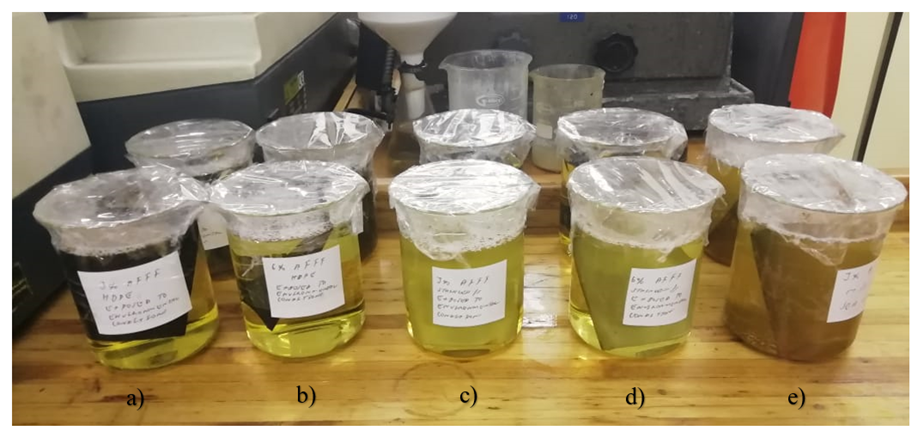
\includegraphics[width=\textwidth]{pureness_of_immersed_afff.png}
    \caption{Pureness of AFFF concentrate after immersion of the materials.}
    \label{ch5:figure:pureness}
\end{figure}

It can be observed from Figure \ref{ch5:figure:pureness} that the pureness of the samples varies greatly. Samples (a-b) are \acrshort{afff} concentrates when \acrshort{hdpe} was immersed, and samples (c-d) are when stainless steel was immersed. It is clear from these samples that there was no significant degradation of the materials immersed. This is because the \acrshort{afff} concentrate was able to maintain its pure yellowish colour during the interaction with these materials. However, when observing closely, it is noticed that samples (a–b) are purer than samples (c–d). This is evidence that stainless steel also underwent the degradation process due to the increase of iron by 55.5 ppm, as suggested by Table \ref{ch5:table:chemical_elements_2}. In contrast, sample (e) is the \acrshort{afff} concentrate when mild steel was immersed. It can be visually observed that mild steel is immensely degraded when it interacts with \acrshort{afff} concentrate. The \acrshort{afff} concentrate's transition from a yellowish to a brownish colour serves as visual evidence of this. This is further justified by the large increase in the iron of 129.5 ppm observed in Table \ref{ch5:table:chemical_elements_2}. Although the precise performance parameters affected by this degradation cannot be concluded, the reaction between mild steel and \acrshort{afff} concentrate remains severe.

\section{Conclusion}
This chapter documented the results obtained using the \acrshort{ftir}, \acrshort{tem}, \acrshort{dls}, and \acrshort{icp-aes} instruments. Tests were conducted to determine the impact of mild steel, stainless steel, and \acrshort{hdpe} on the performance parameters of \acrshort{afff}. The analyses entangled the function groups, particle shape, and size distribution, as well as the elemental composition of \acrshort{afff} concentrate. Most of the tests conducted can be classified as successes concerning reliability. For each test, the results are illustrated in the form of graphs, pictures, calculations, or tables, as well as a discussion of any relevant observations or concerns arising from the results. \acrshort{afff} performance parameters such as foam ability, foam stability, surface tension, foam drainage, and viscosity were all found to be statistically significant during the analyses. Among the three materials tested, mild steel was found to have the greatest impact on \acrshort{afff} performance parameters. While stainless steel was the second ‘severe’ material, \acrshort{hdpe} was the compatible material with only the ESC concerns.